\documentclass[]{article}
\usepackage{tikz-qtree-compat}
\usepackage{tikz}
\usepackage{stmaryrd}
\usepackage{gb4e}

\begin{document}

\begin{exe}
\ex{Ann dances.}
\end{exe}

\begin{exe}
\ex
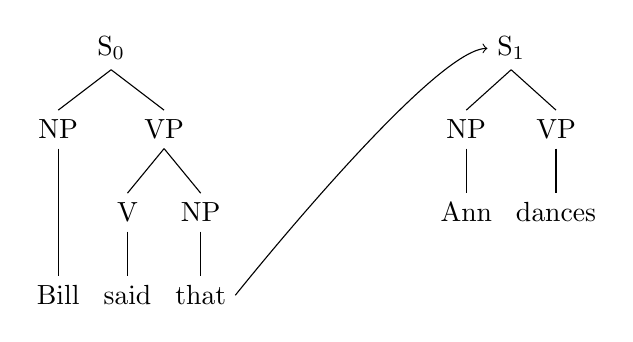
\begin{tikzpicture}[baseline=(current  bounding  box.center)]
\Tree [.S_0 [.NP [Bill ] ] [.VP [.V said ] [.NP \node(a){that}; ] ] ]
\begin{scope}[shift={(2in,0in)}] 
\Tree [.\node(b){S_1}; [.NP Ann ] [.VP dances ] ]
\end{scope}
\draw[->](\subtreeof{a}.0) .. controls +(west:0) and +(west:1) .. (b);
\end{tikzpicture}
\end{exe}


\begin{exe}
\ex
$\left\llbracket
\begin{array}{l}
\Tree [ .S [.NP [.N Ann ] ] [.VP [.V dances ] ] ]
\end{array}
\right\rrbracket$
\end{exe}

\end{document}